\section{Implementierung}

\begin{figure}[h]
 \centering
 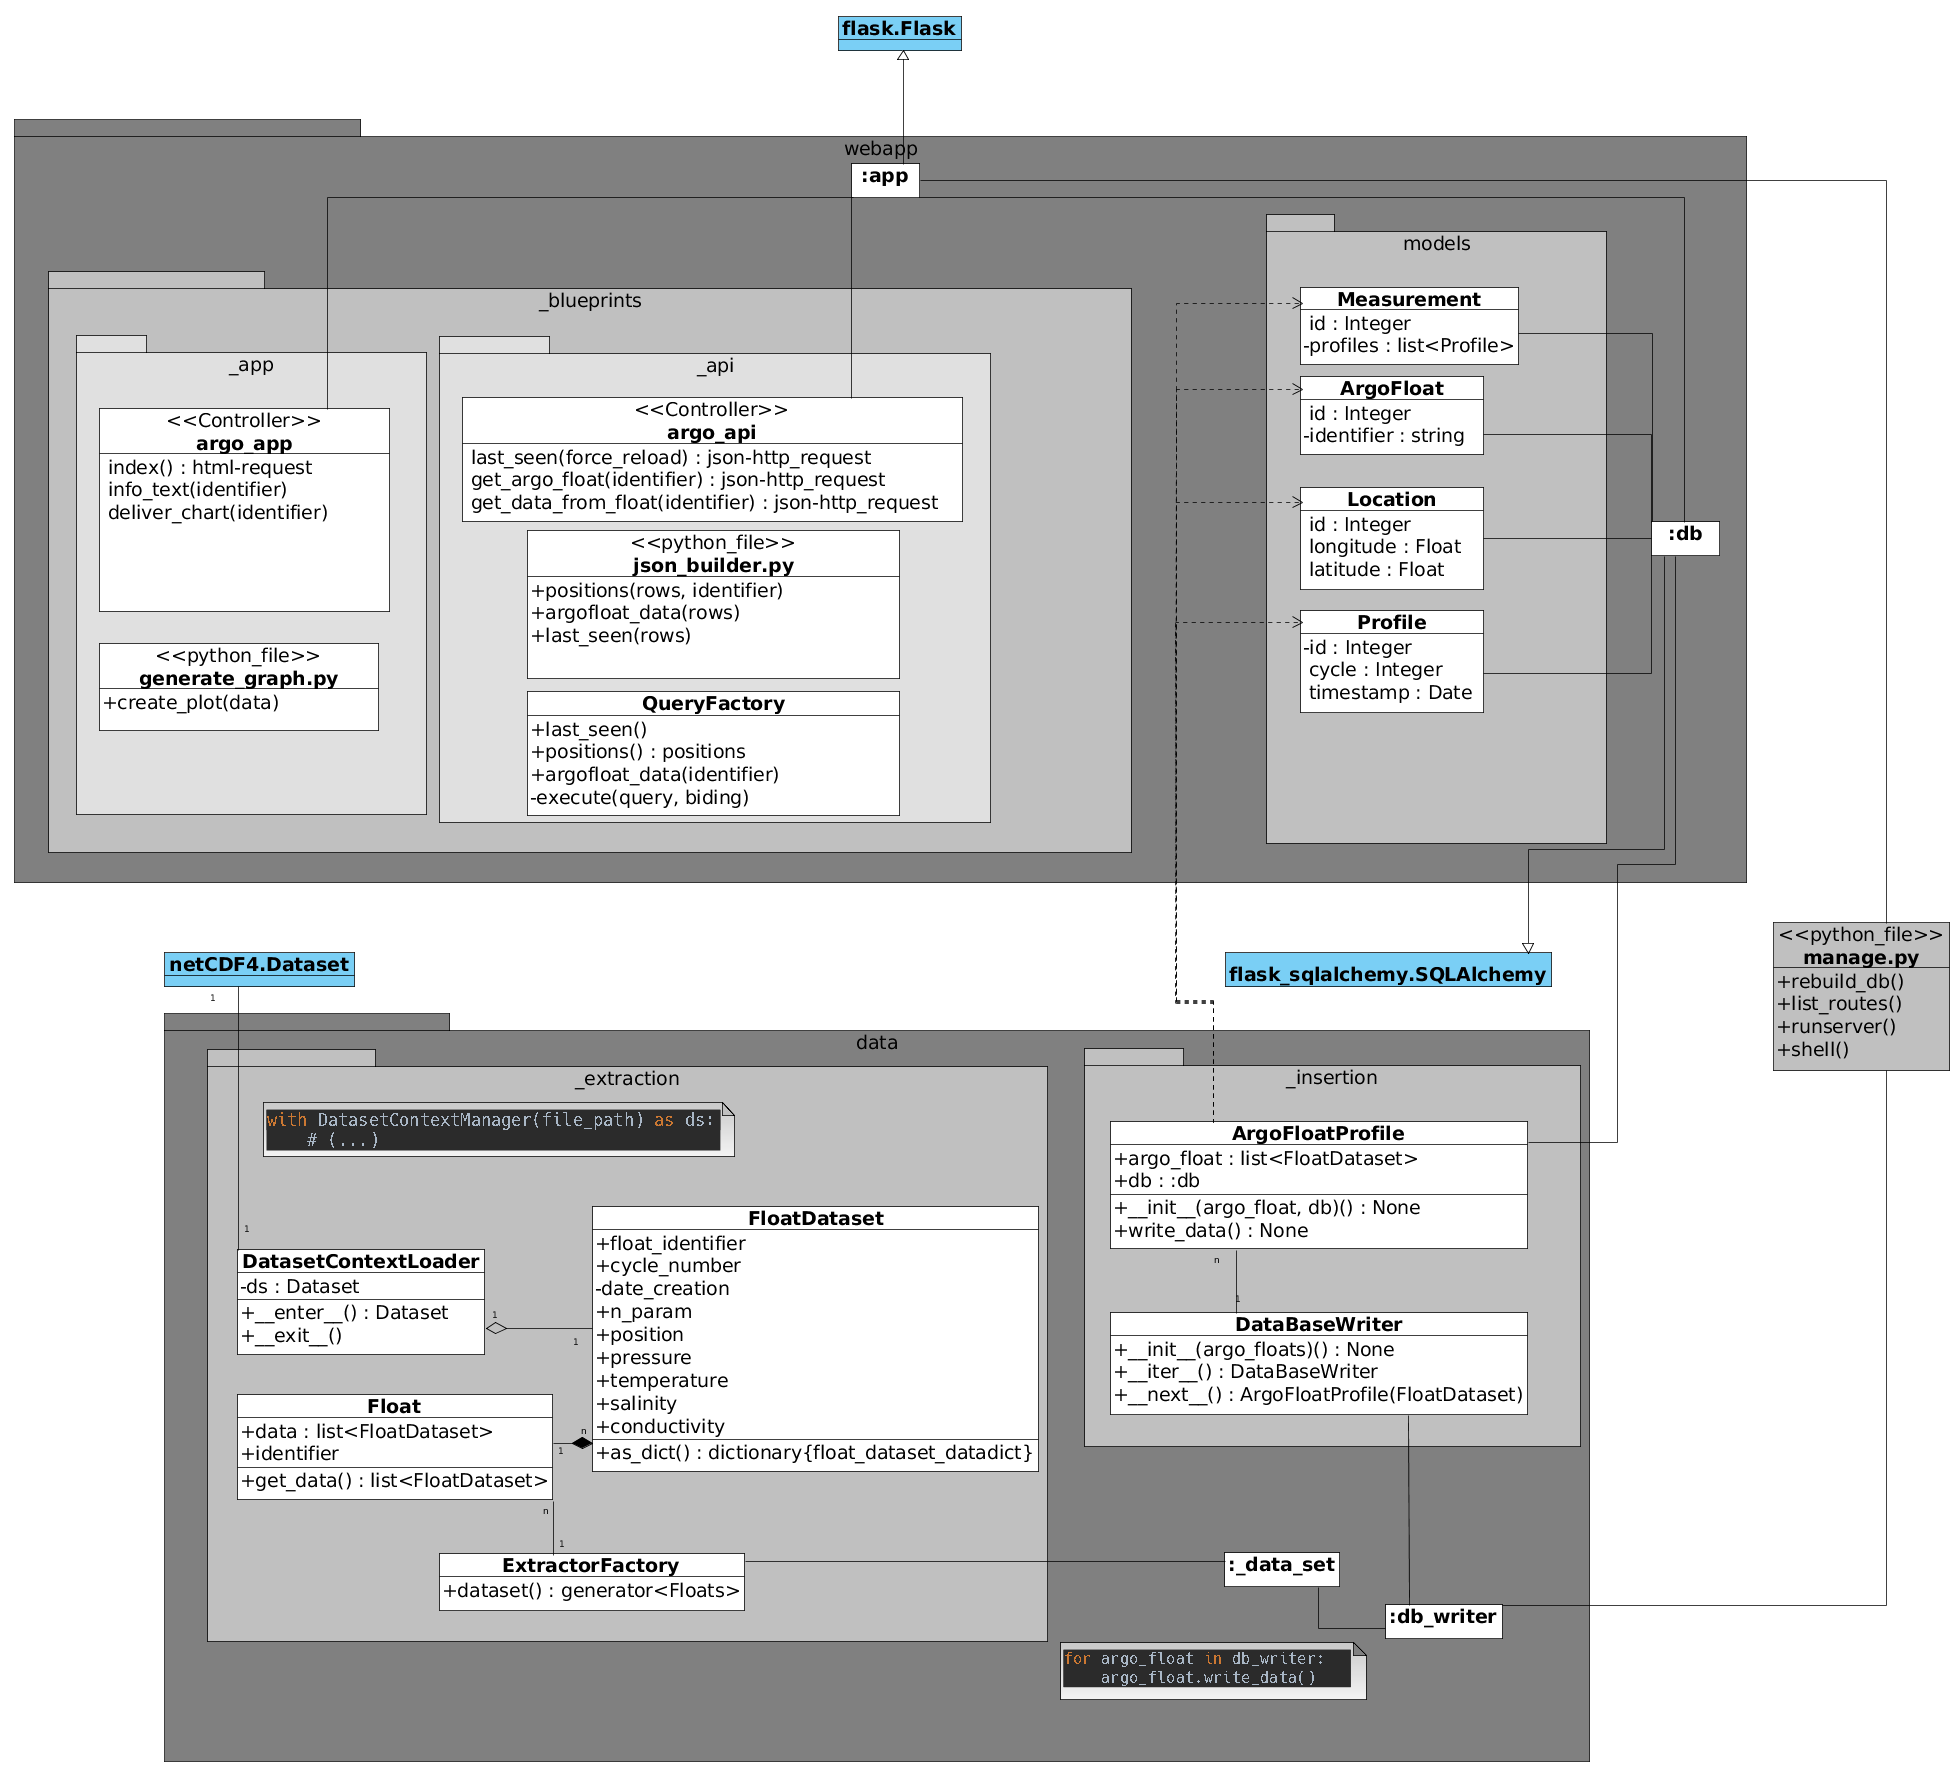
\includegraphics[width=\textwidth]{pix/Modulschema_komplett.png}
 % Modulschema_komplett.png: 876x911 px, 96dpi, 23.17x24.10 cm, bb=0 0 657 683
 \caption{Architekturbeschreibung}
 \label{fig:modulschema}
\end{figure}


% BEGIN DATENAGGREGATION
\subsection{Datenaggregation}

Bei der Aggregation der Daten aus dem Argo Programm sind Schnittstellen auszuarbeiten. Diese Implementierung ist im folgenden beschrieben. 

\paragraph{Dateninput}

Der Datensatz besteht vor der Verarbeitung aus zahlreichen Dateien. Da die Gefahr besteht, dass geöffnete Dateien nicht wieder ordnungsgemäß geschlossen werden, muss eine Schnittstelle geschaffen werden, die unsachgemäße Verwendung der Dateien verhindert. 

Python sieht für diesen Zweck den Kontextmanager vor.

\pythonexternal[%
        caption={Implementierung des Kontextmanagers zur Sicherstellung der richtigen Dateibehandlung.}%
        label=lst:iteratorimpl]{./scr/beispiele/contextmanager.py}



\paragraph{Steuerung}

Um die Verarbeitung der Daten sowie den Prozess der Aggregation in der Datenbank richtig zu modellieren, ist es sinnvoll, den Prozess als Sequenz zu modellieren. Dies erlaubt es, die Datenstruktur über einen Generator vorzuhalten. Python sieht dafür den Iterator vor.

Die hier verwendete Implementierung ist in Listing \ref{lst:iteratorimpl} zu sehen. Das Interface wird über die Funktion \pythoninline{def __next__(self)} in Zeile 12 realisiert. 
Dieses delegiert die Iteration zum Objekteigenen Generator \pythoninline{self.argo_floats}. In dem Moment, in dem ein Objekt aus dem Generator verarbeitet wird, findet die Verarbeitung der dem zugrunde liegenden Datenstruktur statt.

In Zeile 14 wird der Datensatz über ein Objekt ausgeliefert, dass es erlaubt, die Daten in die Datenbank zu überführen.

Damit ist sichergestellt, dass der Prozess nur als Sequenz verwendet werden kann.

\pythonexternal[%
        caption={Implementierung des Iterators zur Steuerung der Aggregationssequenz}%
        label=lst:iteratorimpl]{../BA_argo_proto/data/_insertion/_database_writer.py}

Die Verwendung der Schnittstelle ist in Listing \ref{lst:iterator_verwendung} zu sehen. Dabei wird die Sequenz in Zeile 3 iteriert um den Datensatz daraufhin über die daraufhin folgende Zeile in die Datenbank zu überführen.

\pythonexternal[%
        caption={Verwendung der Schnittstelle zur Steuerung der Datenaggregation}%
        label = lst:iterator_verwendung]{./scr/beispiele/lst-iterator-verwendung.py}
    
    
    
Eine zentrale Problemstellung im Prozess der Überführung der Daten in das Relationale Schema ist die effektive Verwendung des flüchtigen Speichers. Eine klassische, sequenzielle Verarbeitung würde die Daten initial auslesen und diese in Gänze im Ram vorhalten bevor diese über den Mapper in die Datenbank überführt würden. Dieser Prozess wurde durch die Verwendung von Generatoren aufgebrochen. In Listing \ref{lst:dataextractor} ist die Implementierung dieser Schnittstelle zu sehen. Da in der Comprehension runde statt eckige Klammern verwendet werden, wird initial nur die logische Struktur als Sequenz vorgehalten. Die inhärenten Float-Objekte des Generators werden zu dem Zeitpunkt erzeugt, wenn diese durch eine Iteration aufgerufen werden. Damit werden die Daten erst zu dem Zeitpunkt ausgelesen wenn diese für die weitere Verarbeitung benötigt werden,
    


Die Methode \texttt{get\_data\_sets()} erzeugt aus jedem Unterordner im definierten Arbeitsverzeichnis ein Float-Objekt und gibt dieses über das Schlüsselwort \texttt{yield} zurück. 

Durch diese Klasse wird somit ein Generator definiert, der es erlaubt, alle im Arbeitsverzeichnis definierten ArgoFloat Datenobjekte bereitzustellen, ohne diese bereits bei der Instantiierung kennen und abarbeiten zu müssen.


\pythonexternal[%
        caption = {Factory zur Extraktion der Datensätze.},%
        label = {lst:dataextractor}
    ]{/home/sebsch/Dokumente/Uni-Workdir/Bachelorarbeit/BA_argo_proto/data/_extraction/_data_extractor.py}

%END


% BEGIN Webapp
\subsection{Webapplikation}

\subsubsection{Objektrelationales Mapping}

% 1. Vorstellung SQL-Alchemy -- warum gewählt; Vor- und Nachteile

Als Objektrelationalen Mapper wurde sich hier für SQLAlchemy entschieden. Diese Software gilt als erprobt und wird bereits in einer Vielzahl von Softwaresystemen eingesetzt. So verwendet unter anderem reddit oder die Mozilla Foundation SQLAlchemy als Schnittstelle zur Datenhaltung. SQLAlchemy wird für die Verwendung in Flask empfohlen und es existiert eine Erweiterung um die Verwendung des Mappers in Flask zu vereinfachen (vgl. \cite{openingtheflask} S. 33). \\
%% TODO Konzepte, Pattern und Nachteile von SQLAlchemy -- Pattern in Grundlagen zu ORM
%           1. LazyLoading
%           2. databinding
%           3. Foreign Key Mapping 
%           4. rollback


% 2. Implementierung von Entitäten, und Relationen 
In SQLAlchemy werden die Tabelleneinträge in Modellklassenabgebildet. In Listing \ref{lst:models_argofloat} ist die Implementierung des Models für eine ArgoFloat-Messtation zu sehen.

\pythonexternal[%                       -> SQLALCHEMY: ArgoFloat
    caption={Modellklasse für ein Argo-Float},%
    label={lst:models_argofloat}]%
    {/home/sebsch/Dokumente/Uni-Workdir/Bachelorarbeit/BA_argo_proto/webapp/models/_argo_float.py}
    
Die Registrierung des Models erfolgt über die Vererbung einer Metaklasse \texttt{db.Model}. Die Eigenschaften der jeweiligen Entitäten werden über Attribute des Objektes implementiert. Diese werden in Instanzen von \texttt{db.Column} transferiert. Dies erlaubt das Festsetzen des Datentyps. So lassen sich auch weitere Dateiattribute, wie der Festlegung des  Primärschlüssels, definieren. Die Attribute werden durch eine Parameterübergabe in den Initiator der Klasse mit Werten versehen.  
Um das Binding zu umzusetzen, wurden Nachfahren der Modellklassen erzeugt. Diese benötigen für die Zuordnung das Attribut \texttt{\_\_bind\_key\_\_}.


Über das Schlüsselwort \texttt{db.relationship} werden Beziehungen beschrieben. In diesem Fall besteht eine $1 - N$ Beziehung ($\mbox{argo\_float} \leftarrow \mbox{measurements}$) zu \texttt{measurements} (Siehe auch Figure \ref{fig:ERM} auf Seite \pageref{fig:ERM}). Als Übergabeparameter wird ein Name für die Beziehung erwartet. Der Parameter \texttt{backref} gibt den Namen der Klasse auf dem Mapper an. Diese Einstellung erlaubt den Aufruf der Beziehung auch in die andere Richtung. Der Parameter \texttt{lazy} definiert die verwendete Strategie für das Lazyloading. In diesem Fall wurde sich für \texttt{'dynamic'} entschieden. Diese Einstellung gibt bei Lesezugriffen ein vorkonfiguriertes Query-Objekt zurück. Dies erlaub das Hinzufügen weiterer Filter, vor dem Zugriff auf die Tabellen. Die durch diese Beziehung verbundene Modellklasse Measurements ist in Listing \ref{lst:models_measurement} zu sehen.

\pythonexternal[%                       -> SQLALCHEMY: measurement
    caption={Modellklasse für eine Messung},%
    label={lst:models_measurement}]%
    {/home/sebsch/Dokumente/Uni-Workdir/Bachelorarbeit/BA_argo_proto/webapp/models/_measurement.py}

Auf dieser Seite der Beziehung   $\left( \mbox{measurement} \to \mbox{argo\_float} \right)$ ungterscheidet sich deren Implementierung. Für die eindeutige Zuordnung des übergeordneten Argo-Floats, wird deren \texttt{id} als Fremdschlüssel registriert. Die Beziehung benötigt neben dem Namen der anderen Seite keine Weiteren Parameter, da die Beziehung bereits konfiguriert worden ist.


% 3. Lesen und schreiben von Daten aus der Datenbank -- Rollbacks 


Das Schreiben von Daten über den Mapper SQLAlchemy ist Teil der Datenaggregation. Der dort implementierte Programmcode ist in Listing \ref{lst:sqlalchemy_write} zu sehen.


\pythonexternal[%                       -> SQLALCHEMY: Schreiben
    caption={Das Schreiben der Daten eines Argo-Floats in die Datenbank},%
    label={lst:sqlalchemy_write}]%
    {/home/sebsch/Dokumente/Uni-Workdir/Bachelorarbeit/BA_argo_proto/data/_insertion/_argo_float_profile_writer.py}


Die hier implementierte Klasse \texttt{ArgoFloatProfile} ist für das Schreiben aller Datensätze eines ArgoFloats zuständig. Diese verwendet für die Zuordnung der Daten die Modell-Klassen aus der Webapplikation. Durch die Methode \texttt{write\_data} werden die Daten des durch \texttt{\_\_init\_\_} übergebenen Datensatzes in die Datenbank überführt.
Um ein dynamisches Binding realisieren zu können, wird der betreffende Parameter \texttt{bind} übergeben. Mithilfe dieses Parameters wird eine Session aufgebaut, welcher das Schreiben in die Datenbank erlaubt, die über das binding definiert ist.

Für jeden Datensatz eine Instanz der betreffenden Modell-Klasse instanziiert. Die dafür benötigten Daten werden aus den Datensätzen des Klasseneigenen Generator-Objektes \texttt{argo\_float} angefordert und als Parameter übergeben.

Der zuvor definierten Session werden nur die Instanzen der \texttt{Profile}-Klassen übergeben. Da alle zum Messprofil gehörenden Modells in diesem Kontext eindeutig sind, kann SQLAlchemy diese selbstständig zuordnen.
Zum Abschluss werden die Daten über \texttt{session.commit()} in die Datenbank überführt.
\texttt{session.rollback()} erlaubt es, die Veränderungen, die innerhalb dieser Session an der Datenbank herbeigeführt wurden, wieder auf den Urzustand zurückzuführen.  \\

SQLAlchemy bietet eine eigene Abfrage-Sprache an. In Listing \ref{lst:sqlalchemyreadquery} ist eine vereinfachte Implementierung der Abfage zur Bestimmung der Positionshistorie einer Argo-Float zu sehen, wie sie auch in der Web-API implementiert ist. 

\pythonexternal[%                       -> SQLALCHEMY: Lesen 1
    caption={Anfragen über SQLAlchemy zum Lesen von Daten},%
    label={lst:sqlalchemyreadquery}]%
    {scr/beispiele/sqlalchemy_read.py}

In diesem Beispiel wird eine Projektion auf Elemente von Attribute von \texttt{ArgoFloat}, \texttt{Location} und \texttt{Profile} angefordert. SQLAlchemy erlaubt die Definition von Joins über mehere Tabellen, diese werden durch die in den Modell-Klassen definierten Beziehungen aufgelöst. Die Selektion erfolgt durch die Methode \texttt{query.filter()}. In diesem Fall werden nur Relationen der Argo-Float mit dem identifier '1900037' ausgewählt. Die Methode \texttt{query.order\_by()} erlaubt das Sortieren der Ergebnisse. In diesem Fall werden die Datensätze durch das Attribut \texttt{Profile.timestamp} chronologisch sortiert.
\\

SQLAlchemy ist auch in der Lage, in SQL-Sprache definierte Anfragen zu verarbeiten. In Listing \ref{lst:sqlalchemyreadSQL} ist eine vereinfachte Implementierung aus der Web-API zu sehen. Diese extrahiert die letzten ÜPositionen mit den dazugehörigen Zeitpunkten aus der Datenbank. 

\pythonexternal[%                       -> SQLALCHEMY: Lesen 2
    caption={Das Ausführen von SQL Anfragen über SQLAlchemy},%
    label={lst:sqlalchemyreadSQL}]%
    {scr/beispiele/sqlalchemy_read_query.py}
    
Über die Methode \texttt{db.engine.execute()} können SQL-Queries direkt verarbeitet werden. Dies hat aber zwei entscheidende Nachteile. Der Query-Dialekt beschränkt die Anfrage auf ein bestimmtes DBMS. Diese Anfrage ist für PostgreSQL entworfen und würde auf einem anderen DBMS nicht funktionieren. Zum anderen würden Eingaben nicht gegen SQL-Injections gesichert werden. Eine Abfrage wie 
\pythoninline{
db.engine.execute('SELECT * FROM argo\_floats WHERE argo_floats.identifier=\%s' \% user\_input)
} würde also unabschätzbare Sicherheitsrisiken mit sich bringen.
\\

% 4. Einbindung von SQLALCHEMY in den Flask Kontext als Beispiel für zeitkritische import in flask



Flask bietet für die Einbindung von SQLAlchemy eine Erweiterung an. 
Durch diese Erweiterung wird eine SQLAlchemy-Instanzdurch ein zentrales und scheinbar globales Objekt (\texttt{db}) repräsentiert. Dies ermöglicht eine einfache Datenabstraktion und ist für Flask typisch. Dieser Mechanismus wird durch die zeitkritische und in ihrem Ablauf fest vorgeschriebene Erstellung von Objekten und Submodulen erkauft.
Dieser Prozess ist bei der Einbindung von \texttt{flask-sqlalchemy} gut sichtbar. Aus diesem Grund wird die Initialisierung dieser Erweiterung hier gesondert dargestellt.

In Figure \ref{fig:sequenzSQLALCHEMY} ist eine sequentielle Darstellung des Prozesses zu sehen und wird im folgenden beschrieben. 

\begin{figure}[H]
 \centering
 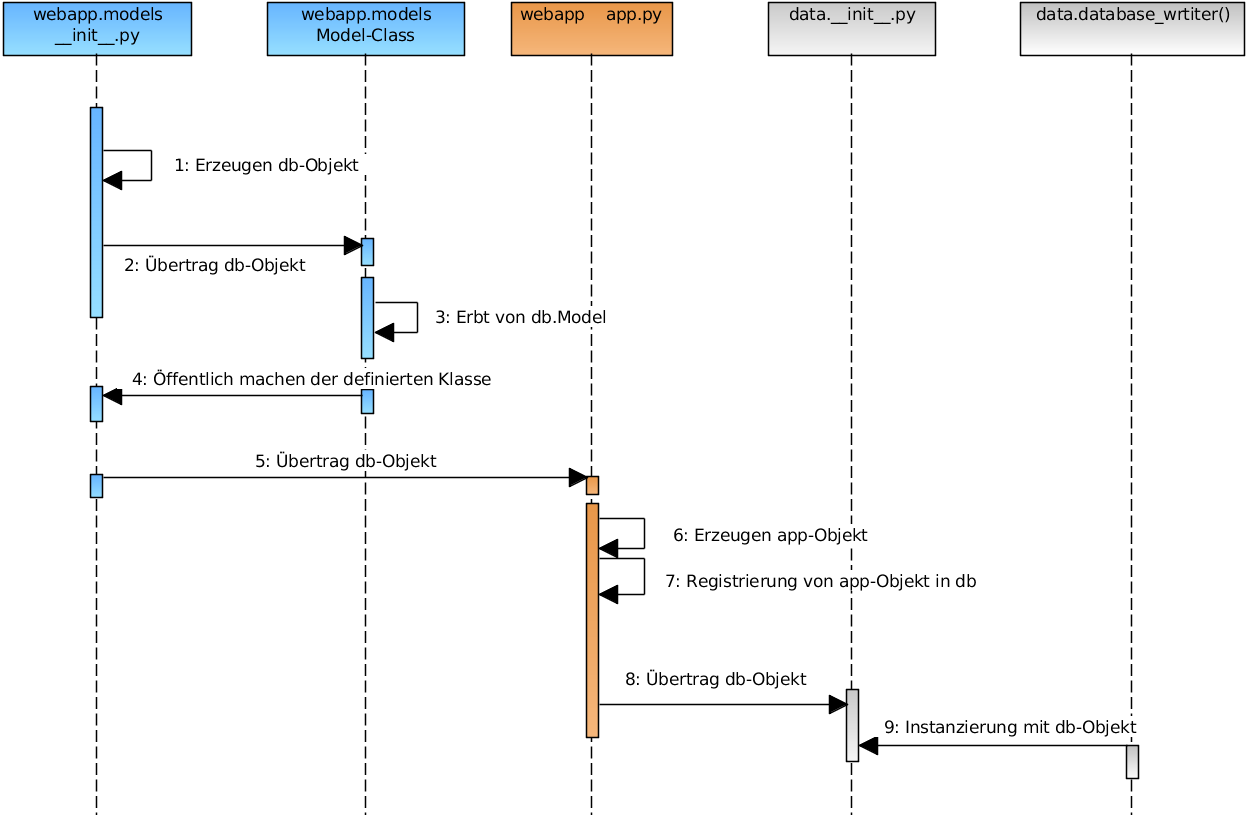
\includegraphics[width=\textwidth]{pix/seq_db.png}
 % seq_db.png: 1310x617 px, 96dpi, 34.66x16.32 cm, bb=0 0 982 463
 \label{fig:sequenzSQLALCHEMY}
\end{figure}


\begin{enumerate}
 \item 
        In der Datei \texttt{webapp.models.\_\_init\_\_.py} muss sichergestellt werden, dass die SQLAlchemy-Instanz noch vor der Initiierung der Modell-Klassen erstellt wurde.
 \item 
        Nun kann das \texttt{db}-Objekt in die Modellklassen übertragen werden. Dafür importieren diese \texttt{db} in ihren Scope.
 \item 
        Die Modell-Klassen werden in \texttt{db} registriert. Dafür erben diese von der Metaklasse \texttt{db.Model}. Siehe auch Listings \ref{lst:models_argofloat} und \ref{lst:models_measurement}.
        
        \pythonexternal[%
    caption={\texttt{webapp.models.\_\_init\_\_.py}},%
    label={lst:initpy_models}]{/home/sebsch/Dokumente/Uni-Workdir/Bachelorarbeit/BA_argo_proto/webapp/models/__init__.py}

    
 \item 
        Die Modell-Klassen dürfen erst nach der Instantiierung von \texttt{db} über den Scope des Submodules heraus bekannt gemacht werden, um sicherzustellen, das dieses bereits existiert. Die Implementierung des Ablaufes ist in Listing \ref{lst:initpy_models} ersichtlich.
 \item  \label{enum:seqdbwebapp1}
        Die Instanz \texttt{db} kann nun mit den in ihr registrierten Modell-Klassen in aus dem Submodul in die Datei \texttt{webapp.\_\_init\_\_.py} importiert werden.

\item   
        Hier wird nun das globale Objekt der Flask-Instanz (\texttt{app}) erstellt und konfiguriert. 
        
        \pythonexternal[%
    caption={ \texttt{webapp.\_\_init\_\_.py}},%
    label={lst:init_webapp}]{/home/sebsch/Dokumente/Uni-Workdir/Bachelorarbeit/BA_argo_proto/webapp/__init__.py}
        
\item   \label {enum:seqdbwebapp3}
        Anschließend wird \texttt{app} in \texttt{db} registriert. Die Schritte \ref{enum:seqdbwebapp1} bis \ref{enum:seqdbwebapp3} können über das Listing \ref{lst:init_webapp} nachvollzogen werden.
        
\item   Die Instanz \texttt{db} aus dem Scope        
        \texttt{webapp.db} ist nun fertig konfiguriert und kann für das Lesen und schreiben in die Datenbank verwendet werden.
\end{enumerate}



\subsubsection{Controller}

% 1. Vorstellung Flask -- warum gewählt; Vor- und Nachteile

  % Blueprints
  

% 2. Trennung von API und APP in verscheidene Blueprints

Die in Kapitel \ref{sec:entwurfRoutes} ausgearbeitete logische Trennung zwischen app und api wird über Blueprints in eigenständigen Python-Modulen realisiert. 

\begin{description}
 \item [argo\_api]
 
    Für die Bereitstellung der Daten benötigt dieses Modul zwei Hilfsprogramme
    
    \begin{description}
     \item [query\_factory] Alle lesenden Zugriffe zur Datenbank werden über dieses Teilprogramm zentral zusammengefasst
         
     \item [json\_builder] Durch dieses Teilprogramm werden die Daten in ein JSON-Format überführt. 
    \end{description}
    
    Der hier definierte controller greift auf diese Hilfsprogramme zu. Die Requests werden über \texttt{flask.jsonify} erstellt.

 
 \item [argo\_app]
\end{description}





% 3. Zentrale Steuerungseinheit via manage.py







\subsubsection{Frontend}

% 1. Verwendete Software -- warum gewähöt; Vor- und Nachteile
% 2. Templatestruktur
% 3. Boostrap 
% 4. openlayers
% 5. Plotting


%END

% 
% % BEGIN SQLALCHEMY
% \subsection{Objektrelationales Mapping}
% 
% 
% 
% 
% 
% 
% Die Einbindung von SQLAlchemy in den Kontext der Webapplikation muss Festgelegten Muster folgen. In Abbildung \ref{fig:sequenzSQLALCHEMY} kann dieser Ablauf über ein Sequenzdiagramm nachvollzogen werden.
% 
% \begin{figure}[!h]
%  \centering
%  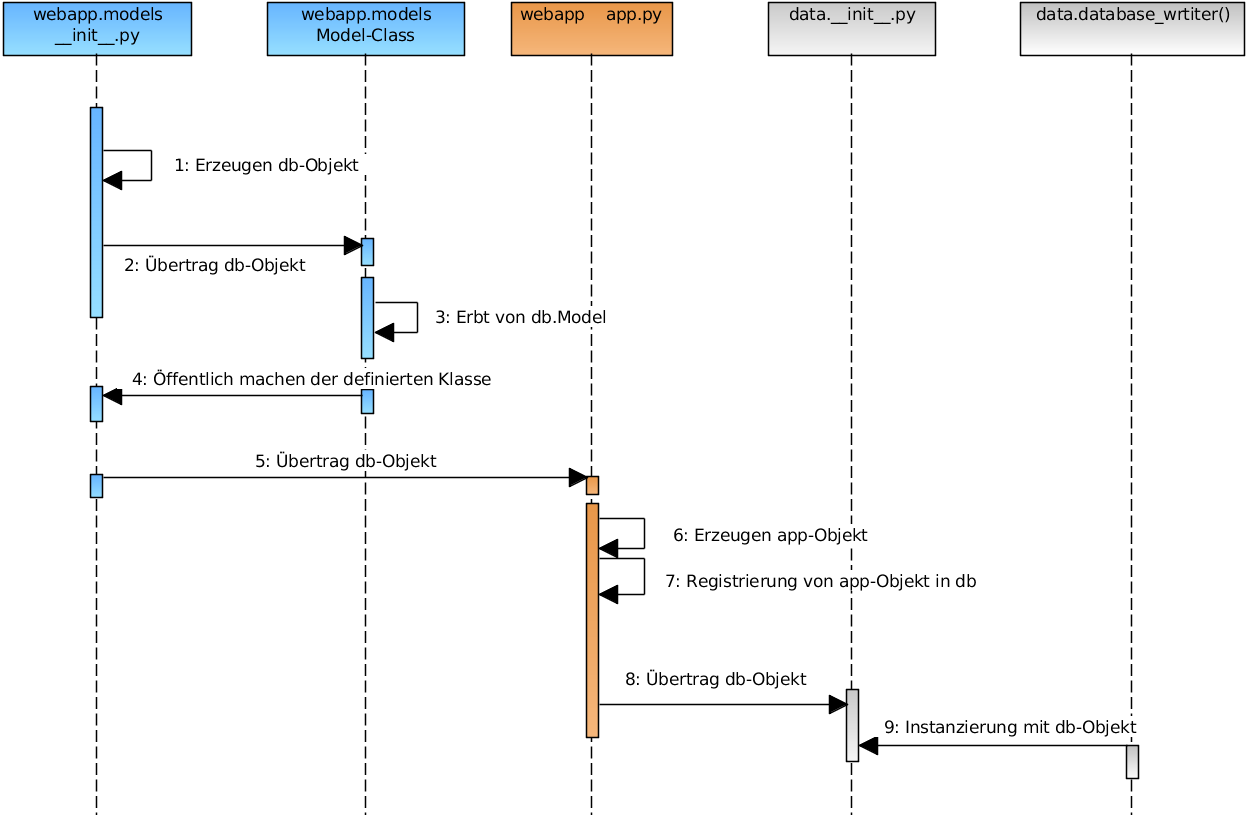
\includegraphics[width=\textwidth]{pix/seq_db.png}
%  % seq_db.png: 1310x617 px, 96dpi, 34.66x16.32 cm, bb=0 0 982 463
%  \label{fig:sequenzSQLALCHEMY}
% \end{figure}
% 
% Die Besonderheit in diesem Prozess besteht darin, das zirkuläre Imports vermieden werden müssen. Daher wird das Objekt für die Verwaltung der Datenbank Schritt für Schritt implementiert.
% 
% Das Objekt von SQLAlchemy wird bei der Erstellung der Models mit erzeugt.
% In Listing \ref{lst:initpy_models} ist dargestellt, auf welche Art die Initialisierung des Moduls \textit{Models} erfolgen kann. 
% 
% \pythonexternal[%
%     caption={Initialisierung der Mpodulstruktur mitsamt SQLAlchemy},%
%     label={lst:initpy_models}]{/home/sebsch/Dokumente/Uni-Workdir/Bachelorarbeit/BA_argo_proto/webapp/models/__init__.py}
%     
% Die Schnittstelle zur Datenbank wird in Zeile 3 über eine Instanz der Klasse SQLAlchemy initialisiert. Diese trägt zu diesem Zeitpunkt noch keinerlei Informationen zu Datenbank oder verwendeter Models.
% Erst nachdem dieses Objekt erzeugt wurde, dürfen die Klassen für die Models in den sichtbaren Bereich des Modules gebracht werden. 
% 
% In Listing \ref{lst:modelArgoFloat} ist exemplarisch die Implementierung des Models für ein ArgoFloat aufgezeigt.
% 
% \pythonexternal[%
%     caption={Implementierung des Modules für eine Entität eines ArgoFloats},%
%     label={lst:modelArgoFloat}]{/home/sebsch/Dokumente/Uni-Workdir/Bachelorarbeit/BA_argo_proto/webapp/models/_argo_float.py}
%     
% In Zeile 1 ist zu sehen, dass die Instanz der Datenbankschnittstelle aus dem Modulkontext geladen wird. Dies wäre nicht möglich, wäre das Objekt noch nicht initialisiert, bevor das Model über die \pythoninline{__init__.py} aufgerufen worden wäre. 
% 
% In Zeile 4 ist zu sehen, das das Model von der Oberklasse \pythoninline{db.Model} erbt. Dadurch wird das in den folgenden Zeilen definierte Model im Kontext der Datenbankschnittstelle registriert und kann nun angesprochen werden. Auf diese Weise werden alle Models an der Schnittstelle registriert. 
% 
% \pythonexternal[%
%     caption={Initialisierung des Modules der webapplikation},%
%     label={lst:init_webapp}]{/home/sebsch/Dokumente/Uni-Workdir/Bachelorarbeit/BA_argo_proto/webapp/__init__.py}
% 
% % END
% 
% 
% \subsection{Controller und Webapplikation}
% 
% Der Controller der Webapplikation teilt sich in zwei Teilbereiche auf.
% Diese Teilbereiche werden über flasks Blueprints realisiert.
% 
% Daten werden über eine API angefragt. Diese sendet bei GET-Requests auf spezifischen URLs JSON-Objekte zurück. Die hierfür benötigten Daten werden über ein Query-Objekt von SQLAlchemy angefragt.
% 
% Der zweite Teilbereich ist für die Darstellung der Applikation. HIer werden zum einen HTML Seiten geredert, aber auch die Bilder für die Graphen-Darstellung erzeugt. Werden hier Daten aus der API benötigt, so stellt diese einen Request an die Seite um das dazugehörige JSON anzufordern.
% 
% \subsection{Frontend}
% 
% 
% 
% 
% 
% 
% 
% 
% 

